\section{Ejercicio 2}
\subsection{Introducci\'on}
En el siguiente apartado se busca analizar la compatibilidad entre compuertas NOR de tecnolog\'ia TTL y CMOS. Para su comparaci\'on se utilizar\'an los integrados 74HC02, 74HCT02 y 74LS02.
\subsection{An\'alisis de datasheet}
Para realizar la comparaci\'on se tomaron los valores de tensiones de entrada y salida para los estados 1 y 0 de las diferentes compuestas, especificados en las hojas de datos (74HC02 \footnote{http://www.ti.com/lit/ds/symlink/sn74hc02.pdf}, 74HCT02\footnote{http://www.ti.com/lit/ds/symlink/sn74hct02.pdf}
y 74LS02\footnote{http://www.ti.com/lit/ds/sdls027/sdls027.pdf}).
\begin{table}[H]
\centering
\begin{tabular}{|c||c|c|c|}
\hline
    & 74HC02 & 74HCT02 & 74LS02 \\ \hline \hline 
$V_{ih}[V]$ & 3,15   & 2       & 2      \\
$V_{oh}[V]$ & 4,4    & 4,4     & 2,4    \\
$V_{il}[V]$ & 1,35   & 0,8     & 0,8    \\
$V_{ol}[V]$ & 0,26   & 0,26    & 0,4    \\ \hline
\end{tabular}
\caption{Margenes de ruido, compuertas NOR}
\label{ej2_table_nor}
\end{table}
Para garantizar la compatibilidad entre dos compuertas se debe cumplir, inicialmente, que $V_{ih} > V_{oh}$ y  $V_{il} < V_{ol}$, observando la tabla \ref{ej2_table_nor} se puede apreciar que en la \'unica combinaci\'on de compuertas que no se cumple esta condici\'on es al cargar una compuerta 74LS02 con una compuerta 74HC02, es decir cargando una compuerta de tecnolog\'ia TTL con una de tecnolog\'ia CMOS que no se encuentre adaptada para tal utilidad, ya que para la compuerta 74HC02 la tensi\'on m\'inima de entrada ($V_{ih}$) para un 1 l\'ogico es de 3.15V lo cual es superior a la tensi\'on de salida m\'ininma ($V_{oh}$) para un 1 l\'ogico del integrado 74LS02.
\subsection{Medici\'on}
Conectando ambas compuertas en cascada y con las entradas cortocircuitadas, para obtener dos compuertas NOT en casacada, se mide la salida de la primer compuerta y la salida de la segundo excitando al circuito con una rampa a fin de poder observar la respuesta en la transici\'on de estados del circuito.
\begin{figure}[H]
\begin{subfigure}{.5\textwidth}
  \centering
  % include first image
  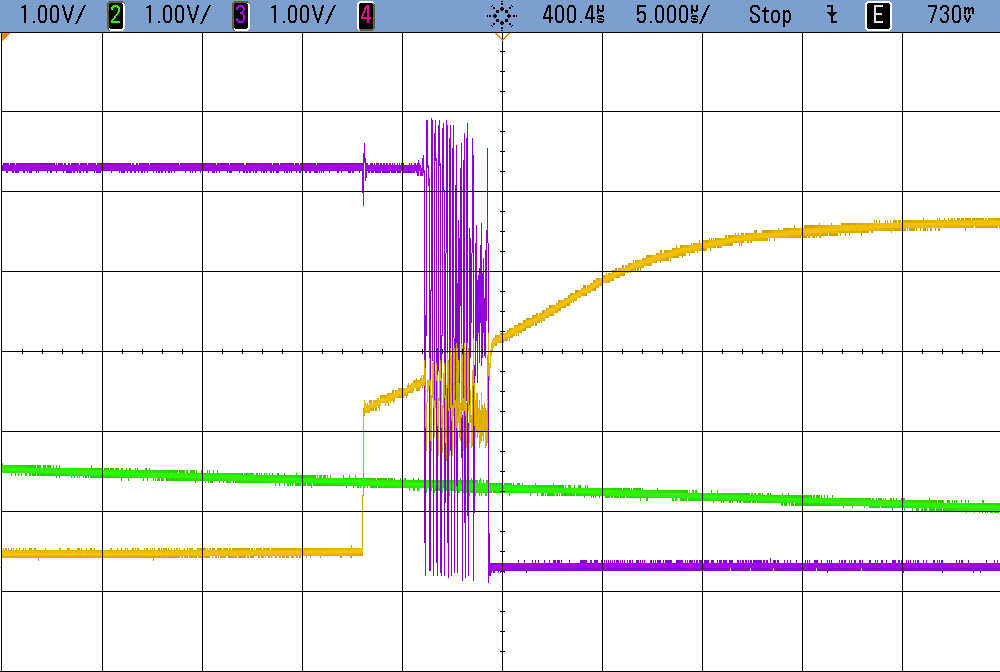
\includegraphics[width=.85\linewidth]{figs/EJ2/LS_HC_0_1.png}  
  \caption{Transici\'on 0-1 de LS.}
  \label{ej2_fig:LS_HC_01}
\end{subfigure}
\begin{subfigure}{.5\textwidth}
  \centering
  % include second image
  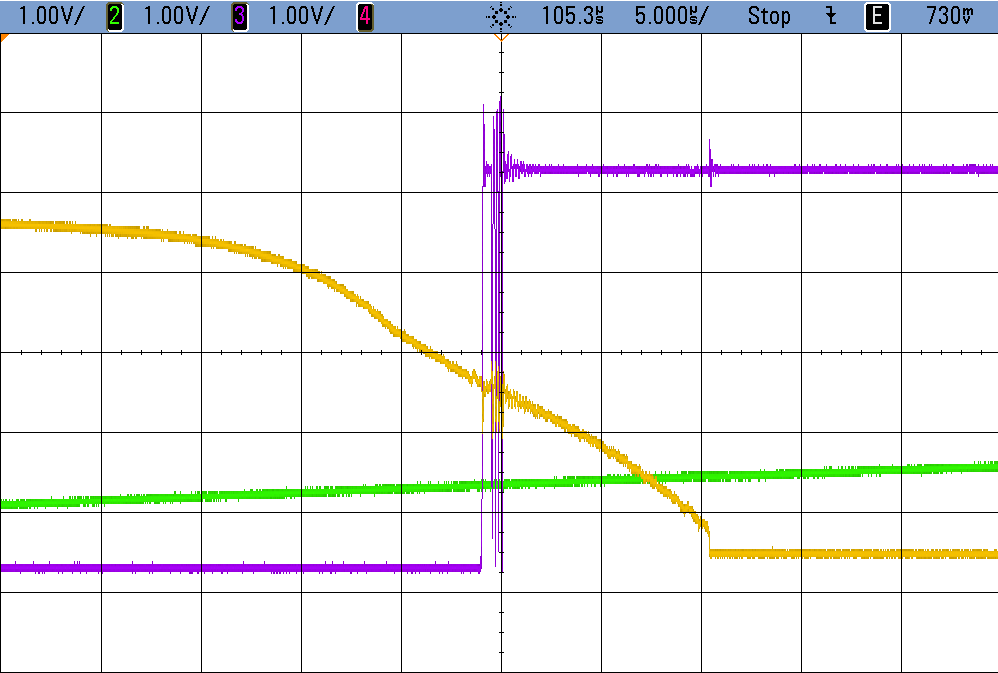
\includegraphics[width=.85\linewidth]{figs/EJ2/LS_HC_1_0.png}  
  \caption{Transici\'on 1-0 de LS.}
  \label{ej2_fig:LS_HC_01}
\end{subfigure}
\caption{Respuesta HC cargando LS.}
\label{ej2_fig:LS_HC}
\end{figure}

\begin{figure}[H]
\begin{subfigure}{.5\textwidth}
  \centering
  % include first image
  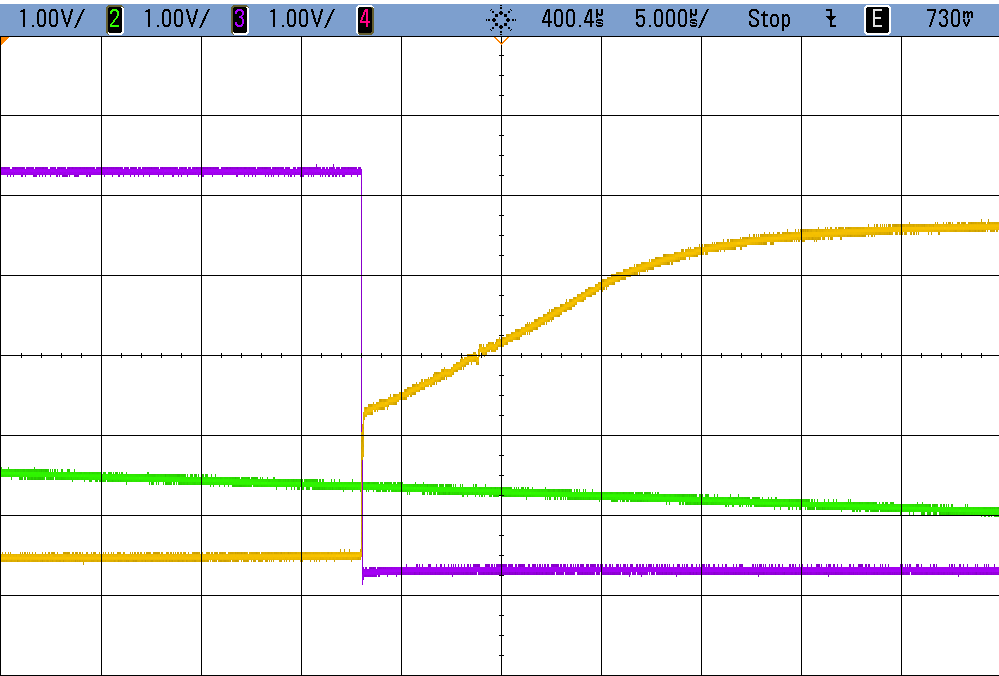
\includegraphics[width=.8\linewidth]{figs/EJ2/LS_HCT_0_1.png}  
  \caption{Transici\'on 0-1 de LS.}
  \label{ej2_fig:LS_HCT_01}
\end{subfigure}
\begin{subfigure}{.5\textwidth}
  \centering
  % include second image
  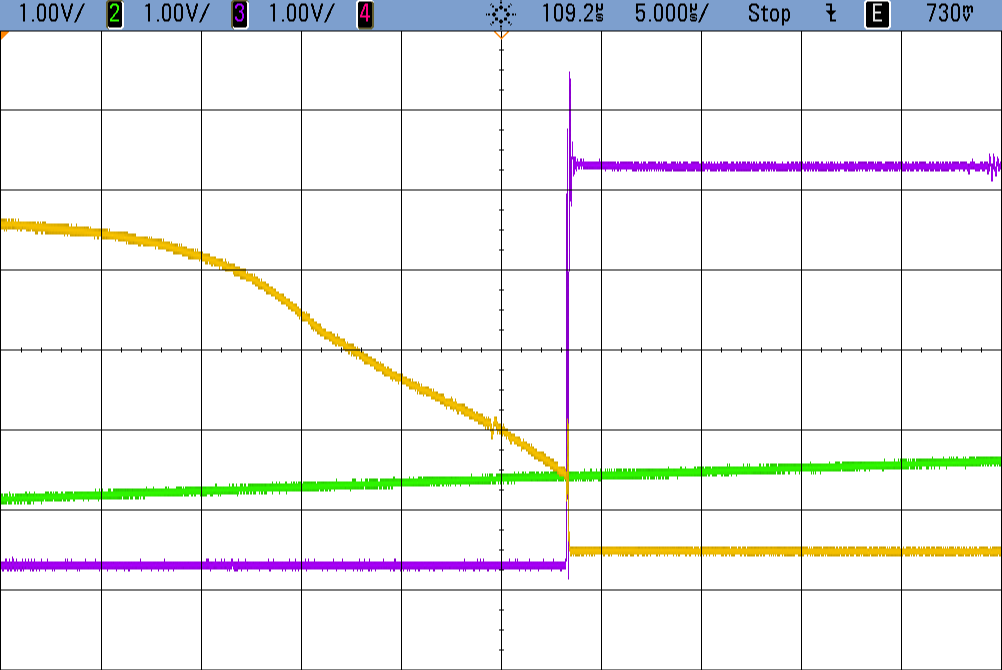
\includegraphics[width=.8\linewidth]{figs/EJ2/LS_HCT_1_0.png}  
  \caption{Transici\'on 1-0 de LS.}
  \label{ej2_fig:LS_HCT_01}
\end{subfigure}
\caption{Respuesta HCT cargando LS.}
\label{ej2_fig:LS_HCT}
\end{figure}

De esta forma se puede ver que al cargar la compuerta LS con la compuerta HC, se presentan oscilaciones debido a la indeterminacion del estado en la compuerta HC, este inconveniete es solucionado en las compuertas de la familia HCT las cuales estan diseñadas para garantizar la compatibilidad con las compuertas de tecnologia TTL que presentan diferentes niveles de ruido.\\
\subsection{Fanout}
Otro aspecto para analizar en la compatibilidad de compuertas es la capacidad de una compuerta de suministrar la corriente que le demanda la carga, ya que de no poder suministrarla adecuadamente, a la salida puede ser malinterpretado el estado l\'ogico.\\
Las compuertas HC02 y HCT02 al pertenecer a la familia de compuertas CMOS demandan corrientes de entrada muy pequeñas, seg\'un las hojas de datos 100nA, lo cual favorece la conexi\'on de estas compuertas como carga de otras compuertas.

